\iffalse
\documentclass[12pt]{article}
\usepackage{graphicx}
\usepackage[none]{hyphenat}
\usepackage{graphicx}
\usepackage{listings}
\usepackage[english]{babel}
\usepackage{graphicx}
\usepackage{caption} 
\usepackage{booktabs}
\usepackage{array}
\usepackage{amssymb} % for \because
\usepackage{amsmath}   % for having text in math mode
\usepackage{extarrows} % for Row operations arrows
\usepackage{listings}
\lstset{
  frame=single,
  breaklines=true
}
\usepackage{hyperref}
\usepackage{mathtools}

%Following 2 lines were added to remove the blank page at the beginning
\usepackage{atbegshi}% http://ctan.org/pkg/atbegshi
\AtBeginDocument{\AtBeginShipoutNext{\AtBeginShipoutDiscard}}


%New macro definitions
\newcommand{\mydet}[1]{\ensuremath{\begin{vmatrix}#1\end{vmatrix}}}
\providecommand{\brak}[1]{\ensuremath{\left(#1\right)}}
\providecommand{\sbrak}[1]{\ensuremath{{}\left[#1\right]}}
\providecommand{\norm}[1]{\left\lVert#1\right\rVert}
\providecommand{\abs}[1]{\left\vert#1\right\vert}
\newcommand{\solution}{\noindent \textbf{Solution: }}
\newcommand{\myvec}[1]{\ensuremath{\begin{pmatrix}#1\end{pmatrix}}}
\let\vec\mathbf


\begin{document}

\begin{center}
\title{\textbf{Convex Optimization}}
\date{\vspace{-5ex}} %Not to print date automatically
\maketitle
\end{center}
\setcounter{page}{1}

\section{12$^{th}$ Maths - Chapter 6}
This is Problem-1(i) from Exercise 6.5
\begin{enumerate}
		\fi
The given function has a minimum value as shown in Figure \ref{fig:12/6/5/1/1/2Fig1}.  
\begin{align}
        \label{eq:12/6/5/1/1/2Eq1}
	f^\prime\brak{x} &= 8x-4 
\end{align}
The minimum value of the function is calculated using Gradient Descent method as below 
\begin{align}
	\label{eq:12/6/5/1/1/2grad_des}
	x_{n+1} &= x_n - \alpha \nabla f\brak{x_n}
\end{align}
Choosing
\begin{enumerate}
\item $\alpha$ = 0.001
\item precision = 0.0000001
\item n = 10000000 
\item $x_0$ = -5 
\end{enumerate}
\begin{align}
	x_{min} &= \frac{1}{2}, f\brak{x}_{min} = 3 
\end{align}
\begin{figure}[!h]
	\begin{center}
		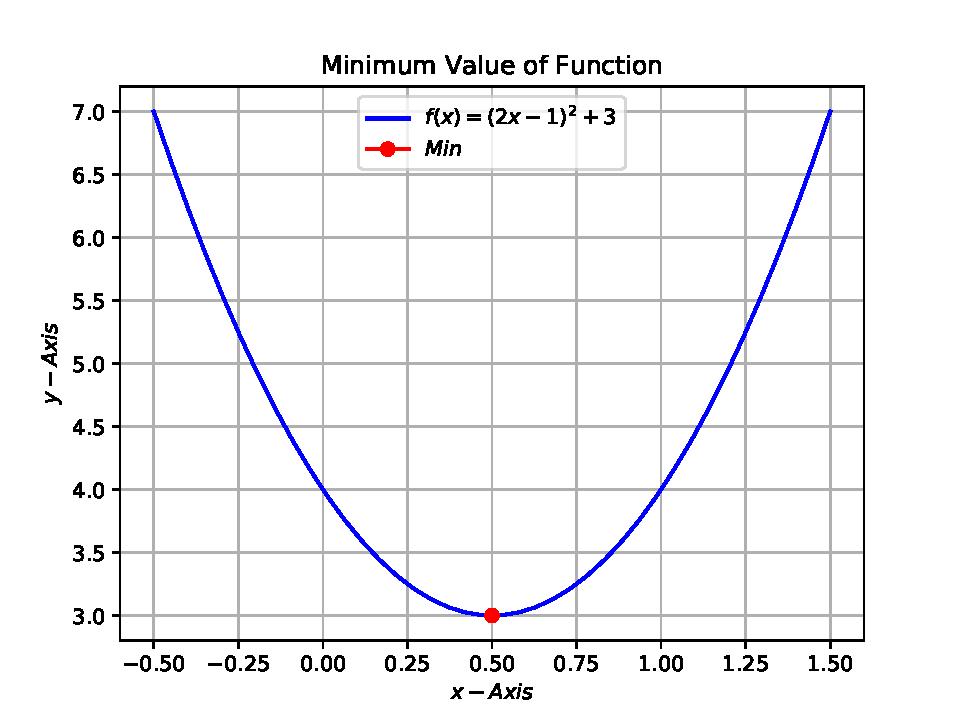
\includegraphics[width=\columnwidth]{12/6/5/1/1/2/figs/Gradient.pdf}
	\end{center}
\caption{}
\label{fig:12/6/5/1/1/2Fig1}
\end{figure}
